\chapter{Measurement of Directional Characteristics I}\label{ax:directional_1}
This appendix serves as a protocol to a series of measurements conducted on the 23\textsuperscript{rd} of February 2018 in the large anechoic chamber (B4-111) at the acoustical lab of Aalborg University at Fredrik Bajers Vej 7.\\
The goal of these measurements was to try out and evaluate a MATLAB-based measurement routine to quantify the directional characteristic of loudspeakers, especially gaining experience with determining the acoustical center of a loudspeaker.

\section*{Measuring Equipment and Materials}
The following measuring equipment was used:
\begin{itemize}[noitemsep]
\item Microphone B\,\&\,K 4144
\begin{itemize}[noitemsep]
\item AAU-number: B4-109-SKF-4
\item Serial number: 297090
\end{itemize}
\item Preamplifier GRAS 26AK
\begin{itemize}[noitemsep]
\item AAU-number: B4-109-SKF-5
\item Serial number: 32811
\end{itemize}
\item Power supply B\,\&\,K 204
\begin{itemize}
\item AAU-number: B4-109-A-1
\item Serial number: 533884
\end{itemize}
\item Calibrator B\,\&\,K 4231
\begin{itemize}[noitemsep]
\item AAU-number: B4-109-A-2
\item Serial number: 2115338
\end{itemize}
\item Power Amplifier Pioneer A-616
\begin{itemize}[noitemsep]
\item AAU-number: B4-109-C-8
\item Serial number: HJ9404841S
\end{itemize}
\item Sound card RME Fireface UCX
\begin{itemize}[noitemsep]
\item AAU-number: 108230
\item Serial number: 23811948
\end{itemize}
\item Turntable: Outline ET 250-3D
\item MATLAB r2017b on OSX 10.11.6
\item Loudspeaker SEAS 33 F-WKA
\end{itemize}

The following material was used:
\begin{itemize}[noitemsep]
%\item \SI{1/2}{\inch} to \SI{1}{\inch} preamp adapter
\item Microphone clip
\item Microphone stand
\item LEMU cable
\item XLR cable
\item Ethernet cable
\item Loudspeaker stand
\item Loudspeaker cabinet, plywood, outside dimensions: (400x400x400)\SI{}{\milli\meter}, wall thickness: \SI{20}{\milli\meter}
\end{itemize}

\section*{Setup}
A sketch of the measurement setup can be found in \autoref{fig:measurement_setup}. A picture is given in \autoref{fig:setup_02_23}

\begin{figure}[htbp]
	\centering
	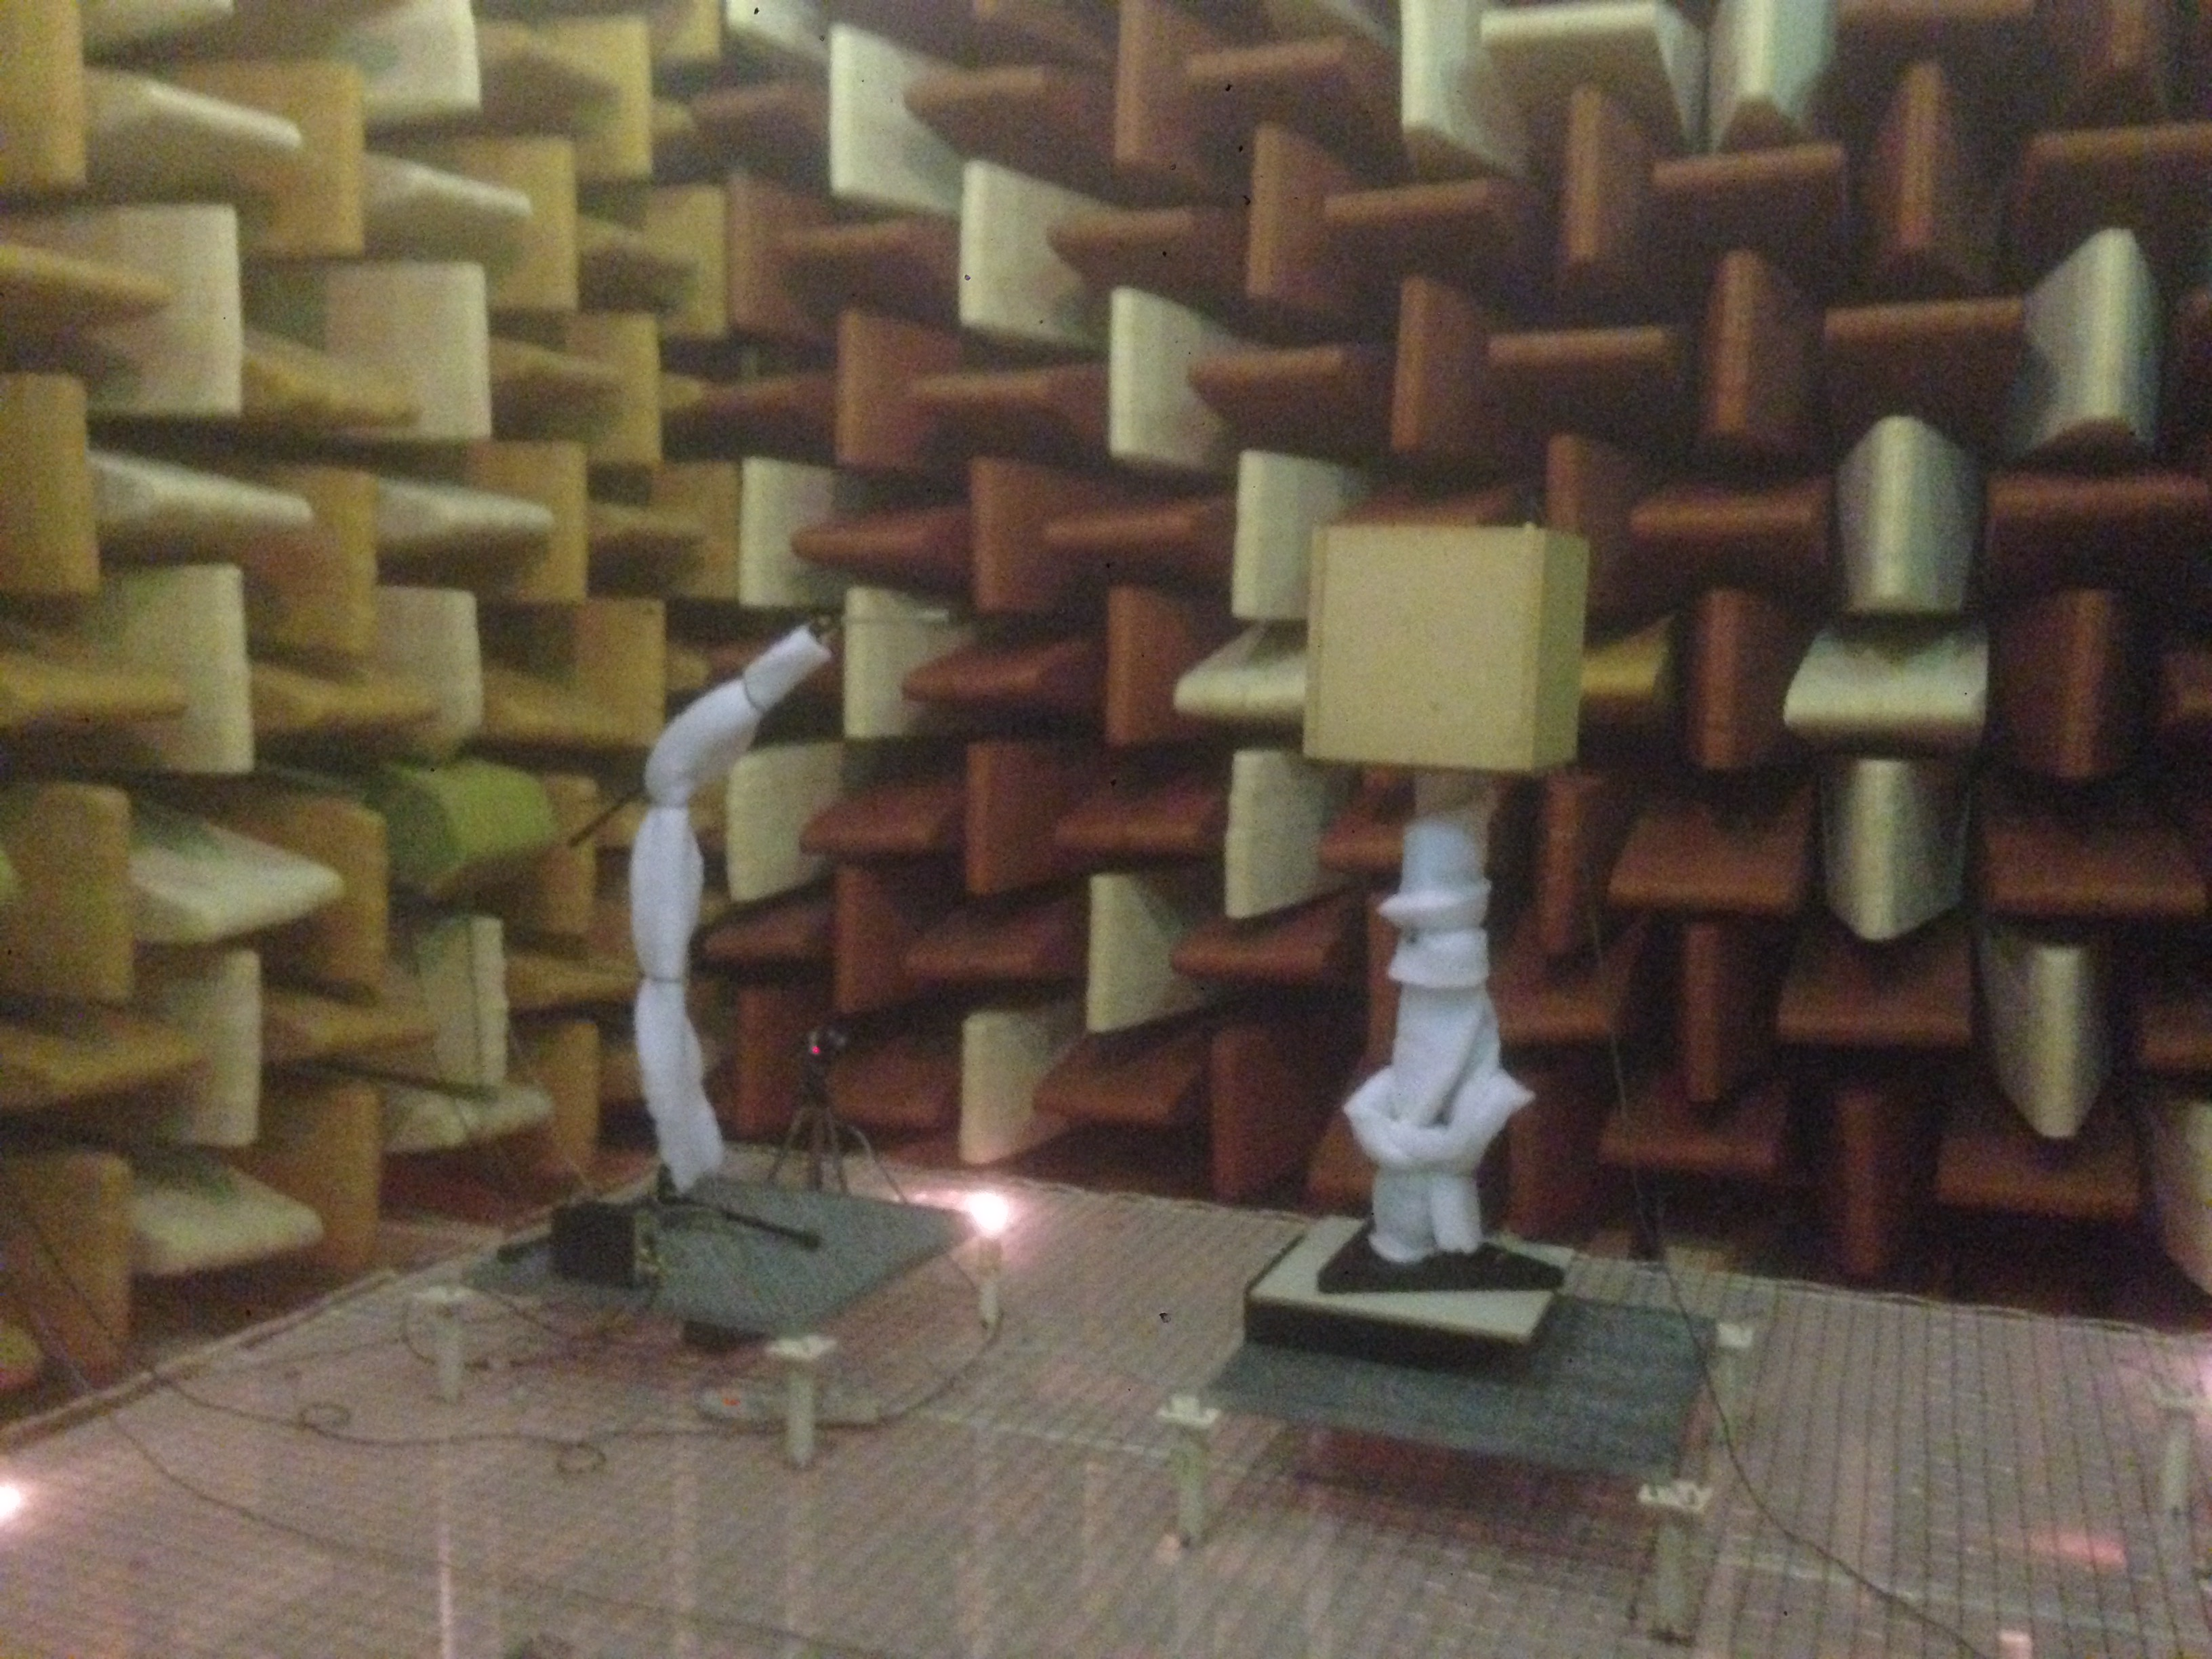
\includegraphics[width=0.7\textwidth]{02_23_setup.JPG}
	\caption{Measurement setup for finding the acoustical center of the speaker.}
		\label{fig:setup_02_23}
\end{figure}

The horizontal distance between the microphone and the edge of the cabinet was \SI{0.75}{\meter}. This rather short distance was deliberately chosen for the sake of determining the acoustic center of the speaker. Directivity measurements should be conducted in the far field, which in the frequency range that this project is about, loudspeaker and microphone have to be placed significantly further apart. 

